% ==========================================================
% =                         ANEXOS                         =
% ==========================================================
%\phantomsection
\section{OLDatasets} \label{appendix:OLDatasets}

Standing for OpenLABEL Datasets, OLDatasets is a custom parser from NuImages format to OpenLABEL format developed in order to integrate it with the \aclink{VCD} library ecosystem developed and maintained by Vicomtech \footnote{\url{https://www.vicomtech.org/en/}}.

\begin{table}[h]
    \centering
    \begin{tabular}{l c c c c}
        \toprule
        \textbf{Name} & \textbf{ID} & \textbf{trainId} & \textbf{Dynamic} & \textbf{Color (RGB)} \\
        \midrule
        background                          & 0  & 0  & False & (0, 0, 0) \\
        animal                              & 1  & 1  & True  & (255, 0, 0) \\
        human.pedestrian.adult              & 2  & 2  & True  & (220, 20, 60) \\
        human.pedestrian.child              & 3  & 3  & True  & (220, 20, 60) \\
        human.pedestrian.construction\_worker & 4  & 4  & True  & (220, 20, 60) \\
        human.pedestrian.personal\_mobility & 5  & 5  & True  & (220, 20, 60) \\
        human.pedestrian.police\_officer    & 6  & 6  & True  & (220, 20, 60) \\
        human.pedestrian.stroller           & 7  & 7  & True  & (220, 20, 60) \\
        human.pedestrian.wheelchair         & 8  & 8  & True  & (220, 20, 60) \\
        movable\_object.barrier             & 9  & 9  & False & (190, 153, 153) \\
        movable\_object.debris              & 10 & 10 & False & (152, 251, 152) \\
        movable\_object.pushable\_pullable  & 11 & 11 & False & (255, 0, 0) \\
        movable\_object.trafficcone         & 12 & 12 & True  & (111, 74, 0) \\
        static\_object.bicycle\_rack        & 13 & 13 & False & (255, 0, 0) \\
        vehicle.bicycle                     & 14 & 14 & True  & (119, 11, 32) \\
        vehicle.bus.bendy                   & 15 & 15 & True  & (0, 60, 100) \\
        vehicle.bus.rigid                   & 16 & 16 & True  & (0, 60, 100) \\
        vehicle.car                         & 17 & 17 & True  & (0, 0, 142) \\
        vehicle.construction                & 18 & 18 & True  & (255, 0, 0) \\
        vehicle.emergency.ambulance         & 19 & 19 & True  & (255, 0, 0) \\
        vehicle.emergency.police            & 20 & 20 & True  & (255, 0, 0) \\
        vehicle.motorcycle                  & 21 & 21 & True  & (0, 0, 230) \\
        vehicle.trailer                     & 22 & 22 & True  & (0, 0, 110) \\
        vehicle.truck                       & 23 & 23 & True  & (0, 0, 70) \\
        vehicle.ego                         & 24 & 24 & True  & (255, 255, 255) \\
        flat.driveable\_surface             & 25 & 25 & False & (128, 64, 128) \\
        \midrule
        ignore                              & 255 & 255 &       &        \\
        \bottomrule
    \end{tabular}
    \caption{Semantic labels defined for NuImages masks}
    \label{tab:semantic_labels}
\end{table}

\begin{figure}[h!]
    \centering
    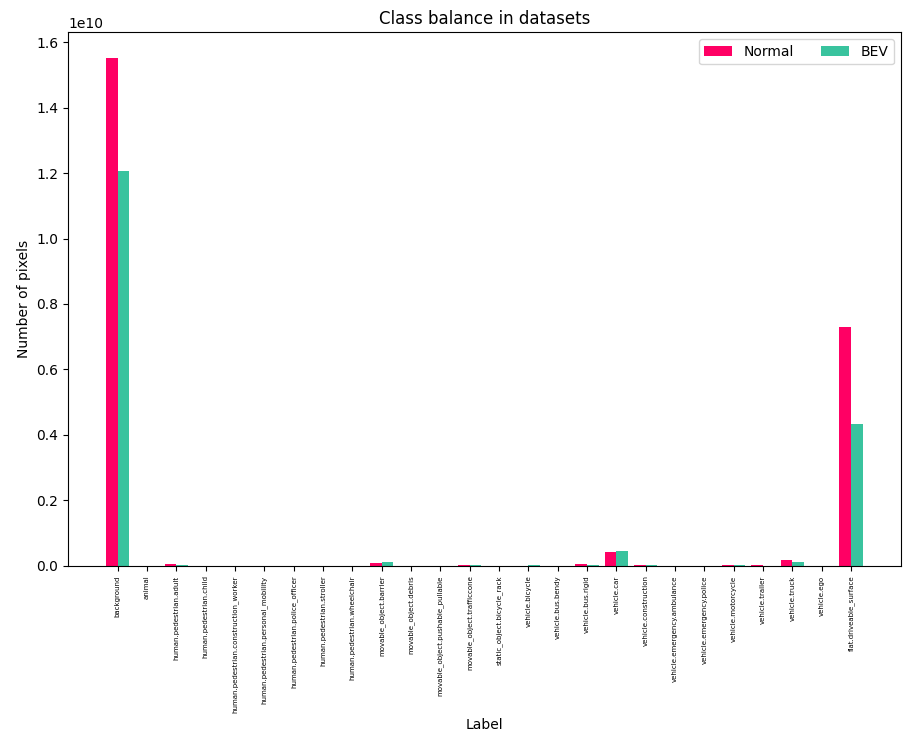
\includegraphics[width=\linewidth]{images/appendix/dataset_class_balance_pixels.png}
    \caption{Number of pixels per class in datasets}
    \label{fig:dataset_class_balance_pixels}
\end{figure}

\begin{figure}[h!]
    \centering
    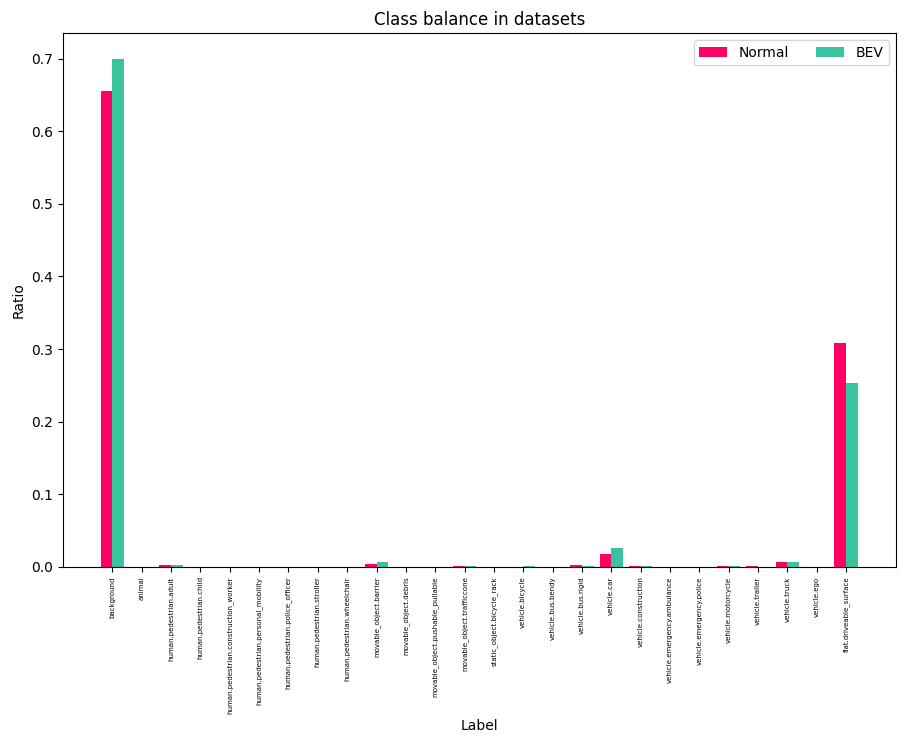
\includegraphics[width=\linewidth]{images/appendix/dataset_class_balance_ratio.png}
    \caption{Relative distribution of classes in dataset}
    \label{fig:dataset_class_balance_ratio}
\end{figure}

% ==========================================================
\section{Rotation matrix to euler angles}
Here \cite{euler_from_matrix} is the pseudocode.

\begin{algorithm}
    \caption{Ground Truth BEV Mask Generation (Single Frame)}
    \label{algorithm:gt_bev_mask}
    \footnotesize

    \begin{algorithmic}[1]
        \State \textbf{Input:} Object data ($objs\_data$), Lane data ($lane\_data$), Scene data ($scene$), FOV coordinate system ($fov\_coord\_sys$), Frame number ($frame\_num$), Ray maximum distance ($ray\_max\_distance$), BEV coordinate system ($bev\_coord\_sys$), Ray step length ($h\_sp$)
        \State \textbf{Output:} BEV Mask ($bev\_mask$)

        \State Initialize camera from $scene$ using $fov\_coord\_sys$ and $frame\_num$
        \State Get camera height ($h$) and width ($w$)
        \State Calculate field of view angle ($\alpha$)

        \State Define ray origin: $rays\_orig \gets [0, 0, 0]^T$
        \State Define ray angles: $rays\_angles \gets$ equally spaced angles from $-\alpha$ to $\alpha$ ($num\_rays$ samples)
        \State Calculate ray directions ($rays\_dirs$) from $rays\_angles$
        \State Define ray steps: $rays\_steps \gets$ equally spaced steps from 0 to $ray\_max\_distance$ ($steps$ samples)
        \State Calculate ray points ($rays\_points$) using $rays\_orig$, $rays\_dirs$, and $rays\_steps$
        \State Transform $rays\_points$ to homogeneous coordinates
        \State Get transformation matrix ($transform\_4x4$) from $fov\_coord\_sys$ to $bev\_coord\_sys$ at $frame\_num$
        \State Transform ray points to $bev\_coord\_sys$
        \State Initialize $intersections$ matrix of size $(num\_rays \times steps)$

        \For{$i$ in $[0, 1, \dots, \text{length}(objs\_data) - 1]$}  \Comment{For each object}
            \State Get bounding box ($bbox$) from $objs\_data[i]$
            \If{$objs\_data[i]$ coordinate system $\neq$ $bev\_coord\_sys$}
                \State Transform $bbox$ to $bev\_coord\_sys$ using $scene$ and $frame\_num$
            \EndIf
            \State Update $intersections$ by checking for intersections between $rays\_points$ and $bbox$  \Comment{Using \texttt{bbox\_intersects\_with\_rays}}
        \EndFor

        \State Identify visible ray points (where $intersections = 0$) and create visible polygons ($visible\_polys$) \Comment{Using \texttt{create\_multipolygon}}
        \State Identify occupied ray points (where $intersections = 1$) and create occupied polygons ($occuped\_polys$) \Comment{Using \texttt{create\_multipolygon}}
        \State Identify occluded ray points (where $intersections = 2$) and create occluded polygons ($occluded\_polys$) \Comment{Using \texttt{create\_multipolygon}}

        \State Define $bev\_height$, $bev\_width$, $bev\_x\_range$, and $bev\_y\_range$
        \State Initialize empty BEV mask ($bev\_mask$)

        \State Get transformation matrix ($lane\_T\_4x4$) for lanes, from 'odom' to $bev\_coord\_sys$ at $frame\_num$
        \For{$k$ in $lane\_data$}  \Comment{For each lane}
          \If{'object\_data' not in $lane\_data[k]$}
                \State Continue  \Comment{Skip if no object data}
            \EndIf
            \State Get lane polygon data ($poly3d\_data$) from $lane\_data[k]['object\_data']['poly3d'][0]$
            \State Assert that polygon is closed
            \State Extract polygon points ($poly3d\_vals$)
            \State Transform $poly3d\_vals$ to homogeneous coordinates
            \State Assert all Z coordinates of lane polygon are 0
            \State Transform lane polygon points to $bev\_coord\_sys$ using $lane\_T\_4x4$
            \State Create lane polygon ($lane\_poly$)
            \If $visible\_polys$ intersects $lane\_poly$
                \State Rasterize $lane\_poly$ and assign 'driveable' label to $bev\_mask$
            \EndIf
        \EndFor

        \State Rasterize $occluded\_polys$ and assign 'occluded' label to $bev\_mask$
        \State Rasterize $occuped\_polys$ and assign 'occuped' label to $bev\_mask$
        \State Color the BEV mask based on labels  \Comment{Using \texttt{target2image}}

        \State \Return $bev\_mask\_colored$
    \end{algorithmic}
\end{algorithm}


% ==========================================================
\section{F1-Score in terms of Intersection Over Union} \label{appendix:f1_iou}
\begin{equation}
    \begin{aligned}
    \text{F1} &= \frac{2TP}{2TP + FP + FN} \\
    \text{IoU} &= \frac{TP}{TP + FP + FN}
    \end{aligned}
    \label{eq:system}
    \end{equation}
    
    % Step 1: Solve F1 in terms of IoU
    \noindent
    We know that:
    \[
    \text{IoU} = \frac{TP}{TP + FP + FN} \Rightarrow TP + FP + FN = \frac{TP}{\text{IoU}}
    \]
    
    Now substitute into the expression for F1:
    \[
    \text{F1} = \frac{2TP}{2TP + FP + FN} = \frac{2TP}{TP + (TP + FP + FN)} = \frac{2TP}{TP + \frac{TP}{\text{IoU}}}
    \]
    
    Factor \(TP\) out of the denominator:
    \[
    \text{F1} = \frac{2TP}{TP \left(1 + \frac{1}{\text{IoU}}\right)} = \frac{2}{1 + \frac{1}{\text{IoU}}}
    \]
    
    Now simplify:
    \[
    \text{F1} = \frac{2\text{IoU}}{1 + \text{IoU}}
    \]
    
    % Step 2: Solve IoU in terms of F1
    \noindent
    Now solve for \(\text{IoU}\) in terms of \(\text{F1}\):
    \[
    \text{F1} = \frac{2\text{IoU}}{1 + \text{IoU}}
    \]
    
    Multiply both sides by \(1 + \text{IoU}\):
    \[
    \text{F1}(1 + \text{IoU}) = 2\text{IoU}
    \Rightarrow \text{F1} + \text{F1} \cdot \text{IoU} = 2 \cdot \text{IoU}
    \]
    
    Bring all terms to one side:
    \[
    \text{F1} = 2\text{IoU} - \text{F1} \cdot \text{IoU}
    \Rightarrow \text{F1} = \text{IoU}(2 - \text{F1})
    \]
    
    Now isolate \(\text{IoU}\):
    \[
    \text{IoU} = \frac{\text{F1}}{2 - \text{F1}}
    \]
    
    \begin{equation}
    \boxed{
    \text{F1} = \frac{2\text{IoU}}{1 + \text{IoU}} \qquad
    \text{IoU} = \frac{\text{F1}}{2 - \text{F1}}
    }
    \label{eq:conversion}
\end{equation}


\section{Merging comparison}

\begin{table}[h]
    \centering
    \tiny
    \begin{tabular}{llcccc}
    \toprule
    \textbf{Merged Class} & \textbf{Original Label} & \textbf{mIoU A} & \textbf{mIoU B} & \textbf{mF1 A} & \textbf{mF1 B} \\
    \midrule
    background & background & 0.98 & 0.98 & 0.99 & 0.99 \\
    \midrule
    animal & animal & 0.00 & 0.00 & 0.00 & 0.00 \\
    \midrule
    human.pedestrian.adult & human.pedestrian.adult & 0.12 & 0.14 & 0.17 & 0.19 \\
     & human.pedestrian.child & 0.00 & - & 0.00 & - \\
     & human.pedestrian.construction\_worker & 0.01 & - & 0.01 & - \\
     & human.pedestrian.personal\_mobility & 0.00 & - & 0.00 & - \\
     & human.pedestrian.police\_officer & 0.00 & - & 0.00 & - \\
     & human.pedestrian.stroller & 0.00 & - & 0.00 & - \\
     & human.pedestrian.wheelchair & 0.00 & - & 0.00 & - \\
    \midrule
    movable\_object.barrier & movable\_object.barrier & 0.11 & 0.17 & 0.13 & 0.21 \\
     & movable\_object.debris & 0.00 & - & 0.00 & - \\
     & movable\_object.pushable\_pullable & 0.00 & - & 0.00 & - \\
     & movable\_object.trafficcone & 0.09 & - & 0.12 & - \\
     & static\_object.bicycle\_rack & 0.01 & - & 0.01 & - \\
    \midrule
    vehicle.car & vehicle.bus.bendy & 0.00 & - & 0.00 & - \\
     & vehicle.bus.rigid & 0.05 & - & 0.06 & - \\
     & vehicle.car & 0.48 & 0.58 & 0.56 & 0.66 \\
     & vehicle.construction & 0.02 & - & 0.03 & - \\
     & vehicle.emergency.ambulance & 0.00 & - & 0.00 & - \\
     & vehicle.emergency.police & 0.00 & - & 0.00 & - \\
     & vehicle.trailer & 0.00 & - & 0.00 & - \\
     & vehicle.truck & 0.14 & - & 0.16 & - \\
    \midrule
    vehicle.ego & vehicle.ego & 0.00 & 0.00 & 0.00 & 0.00 \\
    \midrule
    vehicle.motorcycle & vehicle.bicycle & 0.02 & - & 0.03 & - \\
     & vehicle.motorcycle & 0.06 & 0.07 & 0.07 & 0.09 \\
    \midrule
    flat.driveable\_surface & flat.driveable\_surface & 0.97 & 0.97 & 0.99 & 0.99 \\
    \bottomrule
     & & 0.12 & 0.36 & 0.13 & 0.39 \\
    \bottomrule
    \end{tabular}
    \caption{Per-class metric comparison between Model A and merged Model B evaluated with normal images}
    \label{tab:merging_comparison_bev}
\end{table}
    
    


% ==========================================================
\section{Color palette}
\begin{table}[h]
    \centering
    \renewcommand{\arraystretch}{1.5} % Increase row height
    \setlength{\tabcolsep}{12pt} % Increase column spacing
    \begin{tabular}{c c}
        \toprule
        \textbf{Hex Code} & \textbf{Color Sample} \\
        \midrule


        \#FF0064 & \cellcolor[HTML]{FF0064} \hspace{2cm} \\
        \#FF62A0 & \cellcolor[HTML]{FF62A0} \hspace{2cm} \\
        \#0277BD & \cellcolor[HTML]{0277BD} \hspace{2cm} \\
        \#2AB0D2 & \cellcolor[HTML]{2AB0D2} \hspace{2cm} \\
        \#7700A0 & \cellcolor[HTML]{7700A0} \hspace{2cm} \\
        \#B200EF & \cellcolor[HTML]{B200EF} \hspace{2cm} \\
        \#00A032 & \cellcolor[HTML]{00A032} \hspace{2cm} \\
        \#03FF52 & \cellcolor[HTML]{03FF52} \hspace{2cm} \\
        \#FF9800 & \cellcolor[HTML]{FF9800} \hspace{2cm} \\
        \#FFB03B & \cellcolor[HTML]{FFB03B} \hspace{2cm} \\
        \#C00071 & \cellcolor[HTML]{C00071} \hspace{2cm} \\
        \#FF37AD & \cellcolor[HTML]{FF37AD} \hspace{2cm} \\
        \#00A697 & \cellcolor[HTML]{00A697} \hspace{2cm} \\
        \#44FFEE & \cellcolor[HTML]{44FFEE} \hspace{2cm} \\
        




        % \#F44336 & \cellcolor[HTML]{F44336} \hspace{2cm} \\
        % \#EF5350 & \cellcolor[HTML]{EF5350} \hspace{2cm} \\
        % \#F1464E & \cellcolor[HTML]{F1464E} \hspace{2cm} \\
        % \#FF9800 & \cellcolor[HTML]{FF9800} \hspace{2cm} \\
        % \#FF0064 & \cellcolor[HTML]{FF0064} \hspace{2cm} \\
        % \midrule
        % \#4CAF50 & \cellcolor[HTML]{4CAF50} \hspace{2cm} \\
        % \#86BB48 & \cellcolor[HTML]{86BB48} \hspace{2cm} \\
        % \#39C39E & \cellcolor[HTML]{39C39E} \hspace{2cm} \\
        % \midrule
        % \#0277BD & \cellcolor[HTML]{0277BD} \hspace{2cm} \\
        % \#0097A7 & \cellcolor[HTML]{0097A7} \hspace{2cm} \\
        % \#2AB0D2 & \cellcolor[HTML]{2AB0D2} \hspace{2cm} \\
        % \#01A1FF & \cellcolor[HTML]{01A1FF} \hspace{2cm} \\
        % \#0073B7 & \cellcolor[HTML]{0073B7} \hspace{2cm} \\
        \bottomrule
    \end{tabular}
    \caption{Color Palette}
    \label{tab:color_palette}
\end{table}
